
%(BEGIN_QUESTION)
% Copyright 2010, Tony R. Kuphaldt, released under the Creative Commons Attribution License (v 1.0)
% This means you may do almost anything with this work of mine, so long as you give me proper credit

Examine this P\&ID for a level control system in a vessel where two different fluids (Feed A and Feed B) are mixed together.  The level control valve (LV) is air-to-open (fail-closed):

$$\includegraphics[width=15.5cm]{i01834x01.eps}$$

Determine the effects of the instrument air supply failing, so that the I/P transducer cannot output any air pressure regardless of the 4-20 mA signal sent to it by the controller.  Assume all loop components are properly configured, that the controller is well-tuned, and that a significant amount of time has passed since the instrument air failure.  Compare these conditions with what they were before the failure:

\begin{itemize}
\item{} Liquid level will: {\it increase} from what it was before, {\it decrease} from what it was before, or {\it remain the same} as before
\vskip 10pt
\item{} Control valve will: {\it open up} further, {\it close down} more, or {\it remain in the same position} 
\end{itemize}

\underbar{file i01834}
%(END_QUESTION)





%(BEGIN_ANSWER)

\item{} Liquid level will: {\bf increase}
\vskip 5pt
\item{} Control valve will: {\bf close down more}

%(END_ANSWER)





%(BEGIN_NOTES)

{\bf This question is intended for exams only and not worksheets!}.

%(END_NOTES)


